\documentclass[conference]{IEEEtran}

\usepackage{epsfig}
\usepackage{fancyvrb}

\DefineVerbatimEnvironment%
  {code}{Verbatim}{numbers=left,numbersep=3pt,frame=lines,%
                   xleftmargin=7pt,fontsize=\footnotesize}




\begin{document}


\title{An OSGi-based Sensor Network for \\ Environmental Monitoring}

\author{\authorblockN{XXX}
\authorblockA{San Francisco State University \\
Computer Science Department \\
1600 Holloway Avenue \\
San Francisco, CA 94132 \\
EMail: XXX@sfsu.edu}}


\maketitle
\begin{abstract}
  Abstract.
\end{abstract}


\section{Introduction}

The introduction should emphasize that we interpret sensor networks in
a different way: our focus is on off-the-shelf, highly specialized
sensors for environmental monitoring. Our focus is end-to-end: how to
collect data from a remote location with no stationary power or
Internet connection and deliver the data in near-realtime to a web
browser. Length: first page (including title and abstract).

\section{Use Case}

Researchers in the geosciences rely on sensor data collected by highly
specialized sensors such as the Seabird or YSI. These sensors are
usually deployed in remote locations that not only make their
maintenance difficult, but also access to their measurements.
Typically the sensors are autonomous in the sense that they can run
for a certain time on battery power and store the measurement data in
internal memory. Only when the sensors are serviced, the measurement
data they have collected since the last servicing are uploaded to a
portable storage device. From there the data can be uploaded to
server. This manual procedure to retrieve sensor data is not only
error prone, but also results in a serious time lag between the time
the sensor performs the measurement and when it becomes available for
further processing. For many applications it would be beneficial to
have near-realtime access to the sensor measurement. Being able to
access data when they become available on the sensor device also
reduces the maintenance overhead.

Start with some related work. Who else has done an OSGi-based
infrastructure for sensor networks? Kleber: I believe you have a few
references. This section should be a combination of a use case (using
the RTC and their YSI sonde as an example) and a requirements
analysis: requirements such as remote management and monitoring
capabilities, time-delayed communication, etc. In this section should
be no mentioned of DSP or OSGi. Length: 1 page.

\section{DSP}

Should describe the OSGi-based NetBEAMS architecture. Total length of
this section: 2 pages.

\subsection{Data Sensor Framework and Platform}

should include a picture of a standalone DSP showing a DC and a DP
(general description only). Explain difference between DSP Framework
and DSP Platform. This section should give a top-level overview.
Subsequent sub-sections should explain certain features of the DSP in
more detail.

\begin{figure}
\centering
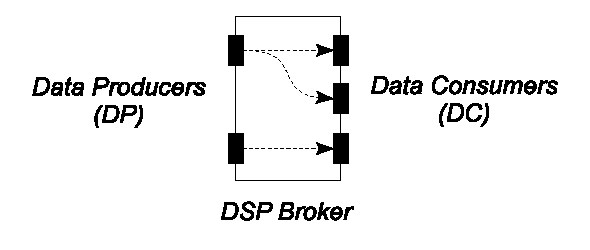
\epsfig{file=dsp, width=7cm}
\caption{\label{FIG_DSP} Data Sensor Platform (DSP).}
\end{figure}

\subsection{DP and DC}

Should give some API sniplets for DP and DC.

\subsection{DSP Message}

Should explain the way DSP Messages are defined: XML Schema and JAXB.

\subsection{Matcher}


\section{NetBEAMS}

Should explain some specific DC and DP we have implemented for
NetBEAMS. Length: 1 - 1.5 pages.

\subsection{YSI Sonde DP}

\subsection{Wire transport DC/DP}

\subsection{Web Managements}


\section{Conclusions and Outlook}

Length (including bibliography): 0.5 pages.

%\bibliography{../literature/lit}
%\bibliographystyle{plain}


\end{document}
